% Compile with XeLaTeX, TeXLive 2013 or more recent
\documentclass{beamer}

% Base packages
\usepackage{fontspec}
\defaultfontfeatures{Scale=MatchLowercase, Mapping=tex-text}

\usepackage{amsfonts}
\usepackage{amsmath}
\usepackage{longtable}
\usepackage{csquotes}
\usepackage{standalone}

\usepackage{graphicx}
\graphicspath{{./images/}}

\usepackage{tikz}
\usetikzlibrary{shapes, calc, arrows, decorations, patterns, chains, fit, petri}
\usetikzlibrary{backgrounds, positioning, decorations.pathreplacing}

\newcommand{\inputpicture}[1]{\input{../pictures/#1}}

\usepackage{tabularx}
\usepackage{multirow}

\usepackage{listings}
\lstset{language=C, basicstyle=\ttfamily, breaklines=true, keepspaces=true, keywordstyle=\color{blue}}

% Setup fonts
\newfontfamily\russianfont{CMU Serif}
\setromanfont{CMU Serif}
\setsansfont{CMU Sans Serif}
%\setmonofont{CMU Typewriter Text}

% Be able to insert hyperlinks
\usepackage{hyperref}
\hypersetup{colorlinks=true, linkcolor=black, filecolor=black, citecolor=black, urlcolor=blue , pdfauthor=Evgeny Yulyugin <yulyugin@gmail.com>, pdftitle=Параллельное программирование}
% \usepackage{url}

% Misc optional packages
\usepackage{underscore}
\usepackage{amsthm}

% A new command to mark not done places
\newcommand{\todo}[1][]{{\color{red}TODO\ #1}}

\newcommand{\abbr}{\textit{англ.}\ }

\newif\ifmipt
\newif\ifsbertech
\input{target}

\ifmipt
\subtitle{Курс <<Параллельное программирование>>}
\fi
\ifsbertech
\subtitle{Курс <<Инфраструктура многопроцессорных систем>>}
\fi
\subject{Лекция}
\author[Евгений Юлюгин]{Евгений Юлюгин \texorpdfstring{\\}{Lg} \small{\href{mailto:yulyugin@gmail.com}{yulyugin@gmail.com}}}
\date{\today}
\pgfdeclareimage[height=0.5cm]{mipt-logo}{common/mipt.png}
\logo{\pgfuseimage{mipt-logo}}

\typeout{Copyright 2014 Evgeny Yulyugin}

\usetheme{Berlin}
\setbeamertemplate{navigation symbols}{}%remove navigation symbols


\title{Параллельные архитектуры}

\begin{document}

\begin{frame}
\titlepage
\end{frame}

\section*{Обзор}

\begin{frame}{На прошлой лекции}
\begin{itemize}
    \item Коллективные операции в MPI
    \begin{itemize}
        \item Синхронизация
        \item Широковещательная рассылка
        \item Распределение и сбор данных
        \item вычислительные операции
    \end{itemize}
\end{itemize}
\end{frame}

\begin{frame}{На этой лекции}
\tableofcontents
\end{frame}

\section{Суперскалер}

\begin{frame}{Суперскалярная архитектура}
Суперскалярный процессор --- процессор, способный запускать несколько команд за
один тактовый цикл.

\vspace*{1cm}\pause
Планирование потока команд происходит динамически в момент исполнения и определяется самим
вычислительным модулем.
\end{frame}

\begin{frame}{Один конвейер --- хорошо, а два --- лучше.}
Один конвейер --- хорошо, а два --- лучше.
\vfill\pause
В процесоре Pentium\textsuperscript\textregistered~было два конвейера:
\begin{itemize}
    \item Главный \textit{u--}конвейер --- выполняет произвольные операции,
    \item Второй \textit{v--}конвейер --- выполняет простые операции.
\end{itemize}
\vfill\pause
При использовании специального компилятора было достигнуто ускорение почти в два
раза по сравнению с Intel\textsuperscript\textregistered~486.
\end{frame}

\begin{frame}{Альтернативы}
Четыре конвейера?
\vfill\pause
Нет. Почему?
\vfill\pause
Слишком громоздкое аппаратное обеспечение. Альтернативы?
\vfill\pause
Один конвейер с большим количеством функциональных блоков.
\end{frame}

\section{VLIW}

\begin{frame}{VLIW архитектура}
VLIW (Very Long Instruction Word) --- архитектура процессоров, в которой каждая
инструкция содержит несколько операций, которые будут выполнены параллельно.

\begin{figure}[htpb]
    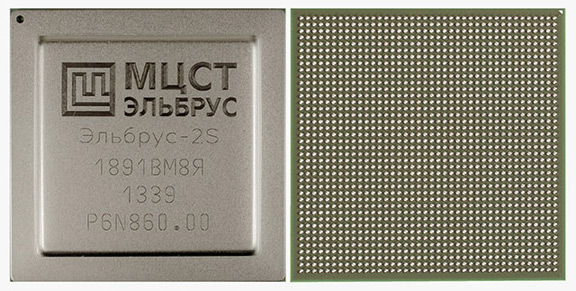
\includegraphics[width=0.7\textwidth]{elbrus-2s}
\end{figure}
\end{frame}

\begin{frame}{Преимущества}
\begin{itemize}
    \item Распределением вычислительных устройств занимается компилятор,
    \item Пониженное энергопотребление, за счет отсуствия узлов, отвечающих за
    распределение задач.
\end{itemize}
\end{frame}

\begin{frame}{Недостатки}
\begin{itemize}
    \item Низкая плотность кода. Большое количество NOP-инструкций,
    \item Увеличенный размер программ,
    \item Сложность программирования на уровне ISA. Только оптимизации
    компилятора.
\end{itemize}
\end{frame}

\begin{frame}{Реализации}
\begin{itemize}
    \item Микропроцессоры серии <<Эльбрус>>,
    \item TriMedia (NXP Semiconductors). 1987--2010 гг.,
    \item Transmeta Crusoe. 2000--2004 гг.
    \begin{figure}[htbp]
        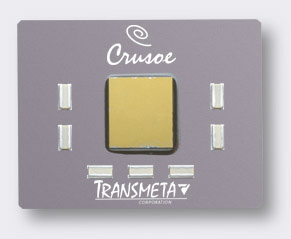
\includegraphics[width=0.4\textwidth]{transmeta-crusoe}
    \end{figure}
\end{itemize}
\end{frame}

\begin{frame}[fragile]{Пример}

Код складывающий 4 числа, находящихся в регистрах R1, R2, R3, R4.

\begin{lstlisting}
R5 = R1 + R2, R6 = R3 + R4;
R0 = R5 + R6, NOP;
\end{lstlisting}

\end{frame}

\section*{Литература}

\section*{Конец}

\begin{frame}[allowframebreaks]{Рекомендуемая литература}
\begin{thebibliography}{99}
    \bibitem{} \textit{Таненбаум~Э.} Архитектура компьютера. --- 5-е изд. ---
        СПб.~Питер, 2007 --- 844~c. ISBN 5-469-01274-3.
    \bibitem{vliw} <<Introduction to VLIW Computer Architecture>>. // Introduction to VLIW Computer Architecture. \url{http://www.psut.edu.jo/sites/qaralleh/CO/CA Documents/11_vliw.pdf}
    \bibitem{patterson-hennessy} \textit{David A. Patterson, John L. Hennessy}. <<Computer Organization and Design, Fourth Edition: The Hardware/Software Interface.>>
\end{thebibliography}
\end{frame}

\begin{frame}{На следующей лекции}
\begin{itemize}
    \item Ускорение и эффективность параллельной программы.
    \item Закон Амдала.
\end{itemize}
\end{frame}

\begin{frame}

{\huge{Спасибо за внимание!}\par}

\vfill

\tiny{\textit{Замечание}: все торговые марки и логотипы, использованные в данном материале, являются собственностью их владельцев. Представленная здесь точка зрения отражает личное мнение автора, не выступающего от лица какой-либо организации.}

\end{frame}

\end{document}
